\documentclass[conference, german]{IEEEtran}
\IEEEoverridecommandlockouts
% The preceding line is only needed to identify funding in the first footnote. If that is unneeded, please comment it out.
\usepackage{amsmath,amssymb,amsfonts}
\usepackage{algorithmic}
\usepackage{graphicx}
\usepackage{textcomp}
\usepackage{xcolor}
\usepackage[utf8]{inputenc}
\usepackage{acronym}
\usepackage{hyperref}
\usepackage[ngerman]{babel}
\usepackage[babel,german=quotes]{csquotes}
\usepackage[backend=biber, natbib=true]{biblatex}
\usepackage{tabularx}
\usepackage{array, multirow} % tabularx: auf Textbreite vergrößern
\usepackage{makecell}
\usepackage{booktabs}
\usepackage{scrextend}
\usepackage{mdframed}
\usepackage{mathtools}
\usepackage{listings}
\usepackage{svg}
\lstset{
	basicstyle=\ttfamily,
	columns=fullflexible,
	frame=single,
	breaklines=true,
	postbreak=\mbox{\textcolor{red}{$\hookrightarrow$}\space},
}
\usepackage[utf8]{inputenc}
\usepackage{minted}
\addtokomafont{labelinglabel}{\sffamily}
\addbibresource{verzechnis.bib}

\begin{document}

\title{Deep Learning\\
{\footnotesize DVA-Seminar 2018}
}
\author{\IEEEauthorblockN{Michael Schwab}
\IEEEauthorblockA{\textit{Fakultät für Informatik} \\
\textit{Hochschule für angewandte Wissenschaften Augsburg}\\
Augsburg, Deutschland \\
michael.schwab@hs-augsburg.de}
}

\maketitle
\renewcommand{\abstractname}{Zusammenfassung}



\begin{abstract}
\end{abstract}

%\begin{IEEEkeywords}
%\end{IEEEkeywords}	
\section*{Lizens}
\href{http://creativecommons.org/licenses/by-nc/4.0/}{
\includegraphics{img/by-nc.png}}\\
{Deep Learning} von {Michael Schwab} ist lizenziert unter einer
\href{http://creativecommons.org/licenses/by-nc/4.0/}{Creative Commons
	Namensnennung-Nicht kommerziell 4.0 International Lizenz}.
\section{Einleitung} 
\section{Konventionen}
\begin{acronym}
	\acro{knn}[KNN]{Künstliches Neuronales Netz}
	\acroplural{knn}[KNNs]{Künstliche Neuronale Netze}
	\acro{dl}[DL]{Deep Learning}
	\acro{ids}[IDS]{Iris-Datensatz}
	\acro{ml}[ML]{Machine Learning}
	\acro{it}[IT]{Informationstechnik}
	\acro{csv}[CSV]{Coma Seperated Values}
	\acro{relu}[ReLU]{Rectified Linear Units}
\end{acronym}
\section{Grundlagen}
\subsection{Grundbegriffe}
\subsection{Datensätze}
Eine essentielle Kompenete des \ac{dl} sind Daten.
Ein Datensatz ist eine Sammlung von Daten in einem gleichen oder ähnlichen Format.
Möchte man \ac{dl} erlernen, steht man oft vor dem Problem keine passenden Daten parat zu haben.
Aus diesem Grund gibt es verschiedene bereits gut klassifizierte Datensätze im Internet zu finden, die den Einstieg in das \ac{dl} erleichtern. 
Ein Beispiel für einen dieser Datensätze ist der \ac{ids}\footnote{\url{https://archive.ics.uci.edu/ml/datasets/iris}}.
\\\\
Der \ac{ids} wurde 1936 von dem Statisker und Biologen Richard Fischer vorgestellt.
Der Datensatz besteht aus 150 Einträgen und umfasst drei verschiedene Gattungen der Iris Blume.
Jeder Eintrag einer einzelnen Blume wird jeweils durch sowohl durch die Blütenkelch Länge und Breite als auch durch die Blütenblatt Länge und Breite beschrieben.
Die drei verschiedenen Gattungen der Iris Blume heißen Iris setosa, Iris virginica und Iris versitosa \citep[vgl.][]{WIKI01}.
\begin{table}
	\caption{Einträge aus dem \ac{ids}}
	\label{table:ids}
	\centering
	\begin{tabular}{c c c c c c}
	\toprule
	{} &    Feature 1 & Feature 2 & Feature 3 & Feature 4 & Label \\
	\midrule
	0 &  5.1 &  3.5 &  1.4 &  0.2 &  Iris-setosa \\
	1 &  4.9 &  3.0 &  1.4 &  0.2 &  Iris-setosa \\
	2 &  4.7 &  3.2 &  1.3 &  0.2 &  Iris-setosa \\
	3 &  4.6 &  3.1 &  1.5 &  0.2 &  Iris-setosa \\
	4 &  5.0 &  3.6 &  1.4 &  0.2 &  Iris-setosa \\
	\midrule
	140 &  6.7 &  3.1 &  5.6 &  2.4 &  Iris-virginica \\
	141 &  6.9 &  3.1 &  5.1 &  2.3 &  Iris-virginica \\
	142 &  5.8 &  2.7 &  5.1 &  1.9 &  Iris-virginica \\
	143 &  6.8 &  3.2 &  5.9 &  2.3 &  Iris-virginica \\
	144 &  6.7 &  3.3 &  5.7 &  2.5 &  Iris-virginica \\
	\bottomrule
\end{tabular}
\end{table}
\\\\
Tabelle \ref{table:ids} zeigt einen Auszug aus dem \ac{ids}.
Anhand diesem Beispiels sollen drei Begriffe erklärt werden, die sehr häufig 
im Bereich des \ac{ml} und \ac{dl} vorkommen.
\begin{mdframed}[backgroundcolor=lightgray]
\begin{labeling}{data}
	\item [Sample] Ein Sample ist ein komplettes Beispiel aus einem Datensatz. 
	In den meißten Fällen ist ein Sample mit einer Reihe in einem Datensatz gleichzusetzen.
	In dem Fall des \ac{ids} entspricht ein Sample einer Blume mit ihren Eigenschaften und ihrer Gattung.
	\item [Feature] Ein Feature ist beschreibt die Eigenschaften eines Samples.
	Im Falle des \ac{ids} hat jedes Sample vier Features.
	\item [Label] Das Label drückt die Art des Samples aus, eine Zugehörigkeit zu einer Klasse.
	Im Falle des \ac{ids} besitzt jedes Sample ein Label. 
	Im ganzen Datensatz gibt es drei Labels, und zwar die drei Blumengattungen.
\end{labeling}
\end{mdframed}

\subsection{Python}
Laut Tiobe Index Juni 2018 ist Python die viert häufigst verwendete Programmiersprache \citep[vgl.][]{TIOBE}. Python gilt als sehr einfach zu lernen und zu schreibende Programmiersprache. Deshalb ist die Python in sehr vielen Disziplienen der \ac{it} vertreten,
besonders auch im Bereich des Scientific Computing. Das die meißten großen \ac{dl}-Frameworks Python als erste Programmiersprache anbieten zeigt, dass Python sich auch hier durchsetzen konnte.
Alle Code-Beispiele in dieser Arbeit sind in Python geschrieben.
\subsection{Python Bibliotheken}
Im Bereich des \ac{dl} gibt es eine Reihe von Python Bibliotheken, deren Einsatz stark zu empfehlen ist:
\begin{mdframed}[backgroundcolor=lightgray]
\begin{labeling}{bib}
	\item [numpy] Numpy ist die Standart Python Bibiliothek für Matrizen Operationen.
	Numpy ist hoch optimiert und extrem schnell. 
	\item [pandas] Pandas ist eine Python Bibliothek Dataframe Objekte zur Verfügung stellt,
	mit denen Daten leicht gelesen, bearbeitet und gespeichert werden können. Unter anderem können \ac{csv} Dateien gelesen werden.
	\item [sklearn] Sklearn ist eine \ac{ml} Python Bibliothek die viele nützliche Funktionen zu dem Vorbereiten und Verarbeiten der Datensätze mitbringt.
	\item [matplotlib] Matplotlib orintiert sich stark an der Programmiersprache Matlab. 
	Mit der Bibliothek Matplotlib können Daten visualisiert werden.
\end{labeling}
\end{mdframed}
\subsection{Deep Learning Frameworks}
TODO
\section{Das Neuron}
TODO
\subsection{Das Perzeptron}
Das Perzeptron bassiert auf der Arbeit von Frank Rosenblatt aus dem Jahr 1958.
Es ist eine einfach Form des Künstlichen Neurons.
Mathematisch lässt sich das Perzeptron wie folgt ausdrücken:
	
	\[
	f(x) = 
	\begin{cases}
	1 & wenn \displaystyle\sum_{i=1}^{m} w_i * x_i + b \\
	0 & andernfalls 
	\end{cases}	
	\]
	
\begin{figure}[H]
	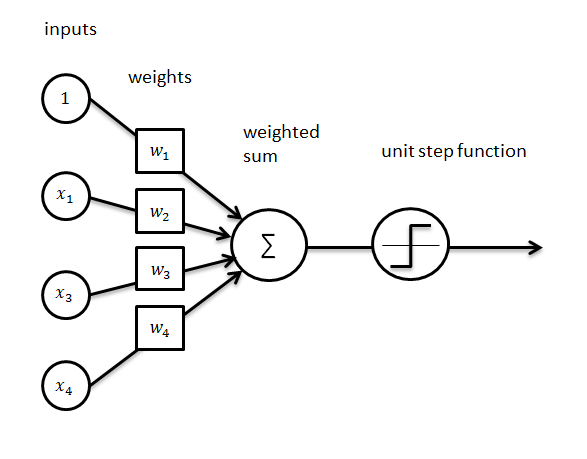
\includegraphics[width=\linewidth]{img/perceptron.png}
	\caption{Schema eines Perzeptrons\citep{ML_PYTHON}}
	\label{fig:perceptron}
\end{figure}	

Das Konzept des Perzeptrons wird im Bild \ref{fig:perceptron} veranschaulicht.
Eine Reihe von Eingabe Werten werden jeweils mit einem Weight multipliziert.
Alle Muliplikationen werden aufsummiert, die Bias Variable addiert. Ist das Ergebnis größer als Null wird eine Eins zurückgegeben, ist es kleiner Null wird eine Null zurückgegeben. Damit kann das Perzeptron zwischen zwei verschiedenen Labels unterschieden, die als Nullen und Einsen Codiert sind. 
\\\\
Die Fähigkeit zu lernen erhält das Perzeptron durch Rosenblatts Perzeptron Lern Algorithmus. Dieser sagt folgendes aus:

\begin{itemize}
	\item Falls die Ausgabe dem erwarteden Wert enstpricht, tue nichts
	\item andernfalls:
	\begin{itemize}
		\item Falls die Ausgabe eine Eins ist, aber eine Null sein sollte:
		dekrementiere die Weights um eine vorher deffinierte Lernrathe.
		\item Falls die Ausgabe eine Null ist, aber eine Eins sein sollte:
		inkrementiere die Weights um eine vorher definierte Lernrathe.
	\end{itemize}
\end{itemize}

Das Perzeptron kann in Python wie folgt umgesetzt werden:

\lstinputlisting[language=Python]{../src/perceptron.py}

Das \textit{Perceptron} Objekt wird mit einer Lern-Rate, einer Input Form und einer Epoch Zahl initialisert. Die Input Form ist wichtig um zu wissen wie viele Weights erzeugt werden müssen, da jeder Input(jedes Feature) mit einer eignen Weight-Variable multipliziert wird. Der Weights Liste in dem Perceptron Objekt wird ein Wert mehr hinzugefügt um die Bias Variable zu simulieren. Die Epochs definieren wie oft über das Datenset iteriert wird. Die \textit{activation\_function} Methode liefert das Ergebnis der \textit{binary\_step} Methode zurück, diese beiden Methoden übernehmen den Aufgabe, die Ausgabe des Neurons in eine Eins oder Null zu quantizieren. 
In der \textit{predict} Methode werden die Eingabewerte mit den Weights multipliziert. Zuvor wird eine Eins in die Eingabewerte eingefügt, um diese mit der Bias Variable multiplizieren zu können, was einer Addition der Bias nach der Muliplikation der Weights entspricht. \\

In der \textit{fit} Methode wird das Perzeptron nun trainiert. 
Zunächst wird über mehrere Epochs hinweg der gesamte Datensatz durchlaufen.
Für jedes Sample wird die Ausgabe des Perzeptrons und das richtige Label verglichen. Falls das Ergebnis von dem Label abweicht, werden die Weights entsprechend der Pezeptron Lern Regel angepasst. Die \textit{learning\_rate} entscheidet hierbei wie stark die Weights angepasst werden. 
Bei einer sehr kleinen Lern-Rate braucht das Perzeptron länger um die Weights optimal anzupassen. Bei einer sehr großen Lern-Rate kann es passieren, dass das Pezeptron über das Ziel hinausschießt. 


\subsection{Das ADALINE}

 


\begin{figure}[H]
	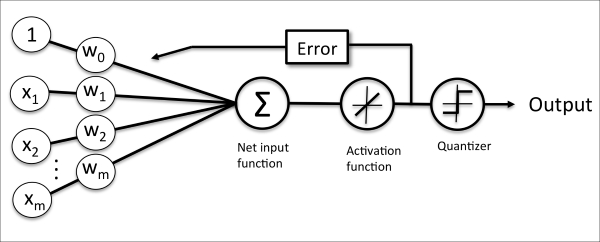
\includegraphics[width=\linewidth]{img/adaline.png}
	\caption{Schema eines ADALINE-Neuron \citep{ML_PYTHON}}
	\label{fig:ada}
\end{figure}

Das ADALINE oder auch Adaptive Linear Neuron ist eine Weiterentwicklung des Perzeptrons. Abbildung \ref{fig:ada} beschreibt den Aufbau eines ADALINE. 
Das ADALINE bietet im Gegensatz zu dem Perzeptron einige Unterschiede wie verschieden Aktivierungsfunktionen, Fehlerfunktionen und Gradient Descent.

Das ADALINE kann in Python wie folgt umgesetzt werden:


\lstinputlisting[language=Python]{../src/adaline.py}

\subsection{Aktivierungsfunktionen}
Eine Aktivierungsfunktion verarbeitet den Ausgangswert der Weights Multiplikation und der Bias Addition. Bisher wurde in dem Perzeptron die Binary-Step oder auch Threshold Aktivierungsfunktion genutzt. Bei der Binary-Step Aktivierungsfunktion wird jeder Wert über Null zu einer Eins und jeder Wert unter Null zu einer Null. Die Binary-Step Funktion ist in Abbildung \ref{fig:binary} dargestellt. 
\begin{figure}[H]
	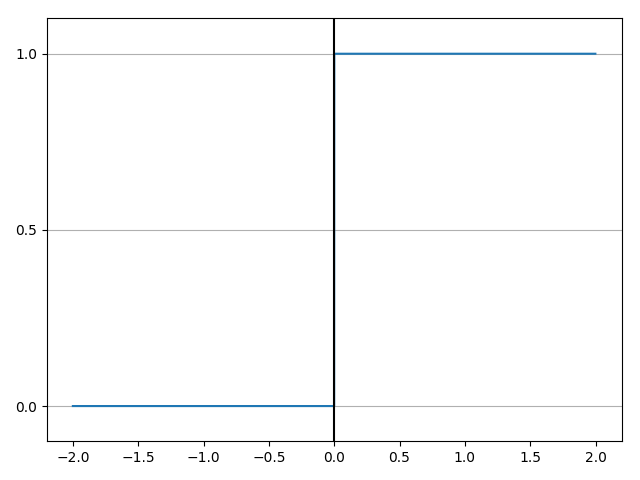
\includegraphics[width=\linewidth]{plots/binary_step.png}
	\caption{Binary-Step Aktievierungsfunktion}
	\label{fig:binary}
\end{figure}

Doch gibt es noch viele weitere Aktivierungsfunktionen. Die wichtigsten sind Sigmoid, \ac{relu} und Tanh.

Die Sigmoid Aktivierungsfunktion ist in Abildung \ref{fig:sigmoid} dargestellt. Mit ihr lassen sich Wahrscheinlichkeiten zwischen zwei Labeln angeben.

\begin{figure}[H]
	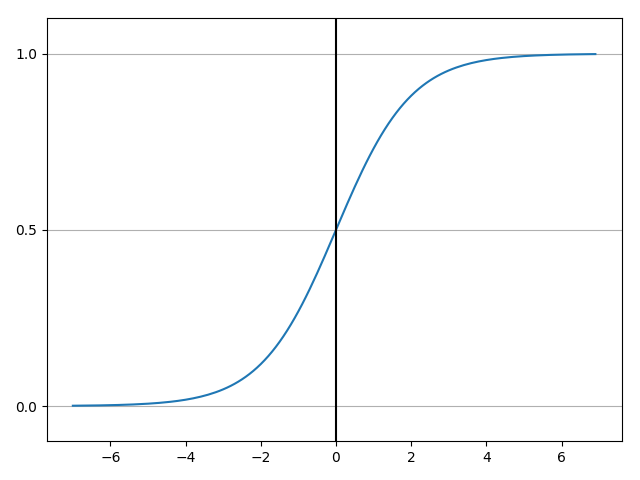
\includegraphics[width=\linewidth]{plots/sigmoid.png}
	\caption{Sigmoid Aktievierungsfunktion}
	\label{fig:sigmoid}
\end{figure}

Ähnlich wie Sigmoid ist die Tanh Aktivierungsfunktion, ihr Ausgabe Wert liegt anders als bei Sigmoid zwischen minus Eins und Eins.
Die Tanh Funktion ist in Abbildung \ref{fig:tanh} abgebildet.

\begin{figure}[H]
	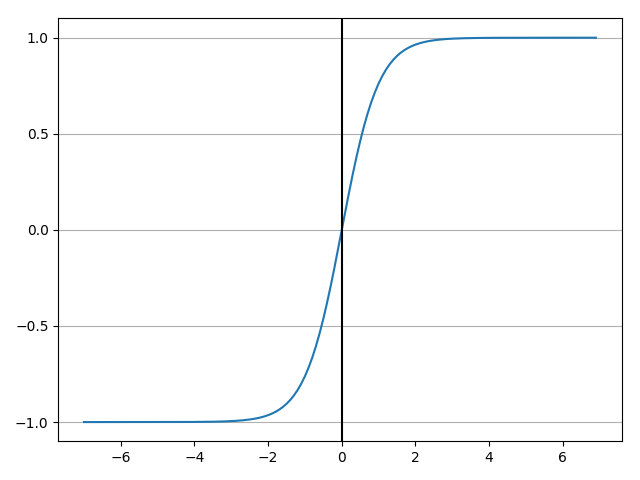
\includegraphics[width=\linewidth]{plots/tanh.png}
	\caption{Tanh Aktievierungsfunktion}
	\label{fig:tanh}
\end{figure}

\ac{relu} ist eine sehr wichtige Aktivierungsfunktion innerhalb von mehrschichtigen Neuronalen Netzen, sie erlaubt es gewisse Verbindungen on Neuronalen Netzen du deaktivieren. Die \ac{relu} Aktivierungsfunktion ist in Abbildung \ref{fig:relu} dargestellt.

\begin{figure}[H]
	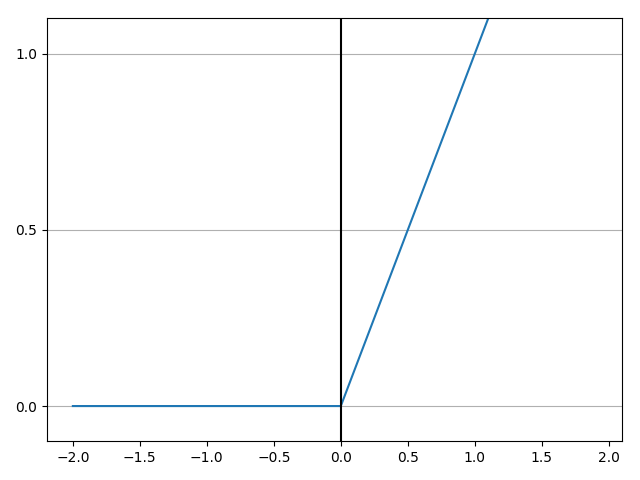
\includegraphics[width=\linewidth]{plots/relu.png}
	\caption{\ac{relu} Aktievierungsfunktion}
	\label{fig:relu}
\end{figure}



\subsection{Fehlerfunktionen}
\subsection{Gradient Descent}
\subsection{Stochastic und Batch Gradient Descent}
\section{Künstliche Neuronale Netze}
\subsection{Definition}
\begin{figure}[H]
	\includesvg[width=\linewidth]{img/not_hidden}
	\caption{\ac{knn}}
	\label{fig:not-hidden}
\end{figure}

\begin{figure}[H]
	\includesvg[width=\linewidth]{img/hidden}
	\caption{Tiefes \ac{knn}}
	\label{fig:hidden}
\end{figure}
\subsection{Arten des Deep Learning}
Im \ac{dl} wird zwischen drei verschiedenen Arten des Lernens unterschieden:
\begin{itemize}
	\item Supervised Learning
	\item Unsupervised Learning
	\item Reinforcement Learning
\end{itemize}
\subsection{Vom Neuron zum Deep Learning}

\lstinputlisting[language=Python]{../src/nn/neural_network.py}

\subsection{Backpropagation}
\subsection{Das Densenet}
\subsection{Das Convolutional Neural Network}
\subsection{Das Recurrent Neural Network}

%\begin{thebibliography}{00}
%\bibitem{b7} M. Young, The Technical Writer's Handbook. Mill Valley, CA: University Science, 1989.	
%\end{thebibliography}
\printbibliography
\end{document}
